%% IEEE Access submission — revision of the IEEE Software desk-rejected
%% manuscript SW-2026-05-0250.
%% Authors: Florin Olariu, Lenuta Alboaie
%% Template: IEEEtran v1.8b, journal mode (no compsoc — IEEE Access default).
\documentclass[journal]{IEEEtran}

% ---------- packages ----------
\usepackage{cite}
\usepackage{amsmath,amssymb}
\usepackage{graphicx}
\usepackage{xcolor}
\usepackage{booktabs}
\usepackage{array}
\usepackage{url}
\usepackage{hyperref}
\usepackage{tikz}
\usetikzlibrary{shapes.geometric, arrows.meta, positioning, fit,
                backgrounds, decorations.pathreplacing}
\usepackage{balance}
\usepackage{listings}
\lstset{basicstyle=\small\ttfamily,breaklines=true,frame=none,
        keywordstyle=\color{blue!70!black},commentstyle=\color{gray}}

% ---------- TBD / TODO markers (visible in draft, removed before submission) ----------
\newcommand{\TBD}[1]{\textcolor{red!80!black}{[TBD: #1]}}
\newcommand{\NEEDDATA}[1]{\textcolor{orange!80!black}{[DATA: #1]}}

% ---------- title block ----------
\title{A Skill-Mediated LLM Workflow for Migrating a .NET Monolith\\
       to Microservices: A Controlled Case Study}

\author{Florin~Olariu~and~Lenu\c{t}a~Alboaie%
  \thanks{F.~Olariu is with the Faculty of Computer Science,
    Alexandru Ioan Cuza University of Ia\c{s}i, Romania, and with
    Suvoda LLC. E-mail: \url{folariu@suvoda.com}}%
  \thanks{L.~Alboaie is with the Faculty of Computer Science,
    Alexandru Ioan Cuza University of Ia\c{s}i, Romania.}%
  \thanks{Manuscript submitted to IEEE Access, 2026.}}

\markboth{IEEE Access, 2026}%
         {Olariu \& Alboaie: A Skill-Mediated LLM Workflow for .NET Migration}

\IEEEtitleabstractindextext{%
% ---------- abstract ----------
\begin{abstract}
Migrating a monolithic application to cloud-deployed microservices is
laborious. Recent LLM-based coding assistants help with isolated steps,
but they do not orchestrate the full sequence --- decomposition,
testing, review, and deployment --- that the migration actually
requires. We report a controlled, multi-case study of one composition
pattern addressing this gap: ten Claude~Code skills chained into a
single end-to-end workflow for migrating .NET monoliths. The primary
case uses \textit{PetRescue}, an ASP.NET~Core~10 monolith, and
produces four public artefacts: the monolith (Slice~1), an
independently-engineered manual microservices reference (Slice~2),
the workflow's automated decomposition (Slice~1~Refactored), and a
Terraform configuration for Oracle Cloud Infrastructure (Slice~3).
A second case --- a transfer check on Microsoft's
\textit{eShopOnWeb} monolith, scored against the active
\textit{dotnet/eShop} microservices reference --- replicates the
primary findings on a substantially different codebase and domain.
On PetRescue, ten repeated runs of the skill-mediated workflow scored
a mean of 12.11 of 20 (60.6\%, $\sigma{=}3.9\%$) on a pre-registered
twenty-dimension structural rubric, with a 10\% skill-invocation
failure rate. Three baseline conditions tease apart what the
skill abstraction contributes from what prompt specificity
contributes. Ten runs of the raw LLM with a fully-specified prompt
(enumerating the intended deliverables) scored 14.80 of 20 (74.0\%,
$\sigma{=}3.2\%$). Five runs of the same model with a deliberately
vague single-sentence prompt --- the matched-specificity baseline,
representing a practitioner who has not invested in prompt
engineering --- scored 12.75 of 20 (63.8\%, $\sigma{=}2.5\%$), with
a 20\% premature-exit failure rate. The skill-mediated workflow is
statistically indistinguishable from the matched-specificity
baseline ($t{=}-1.77$, $p > 0.1$). The original 13.4 percentage-point
skill-vs-baseline gap therefore decomposes into a 10.3-point
prompt-specificity effect ($t{=}-6.40$, $p<0.001$) and a 3.2-point
skill-abstraction effect that does not reach significance. On
eShopOnWeb (transfer case), three skill-mediated runs and three
fully-specified baseline runs reproduce a $-13.3$-point gap that
matches PetRescue's $-13.4$-point gap to within 0.1 percentage
points: the prompt-specificity effect transfers across codebases. The
workflow's automated security checks exhibit perfect recall (10/10
flagged) but 52.6\% precision and 10\% specificity on a matched
ten-clean, ten-vulnerable corpus, consistent with automated DevOps
hygiene rather than formal security validation. We interpret these
findings honestly. The skill abstraction is approximately as good
as a vague-prompt baseline on single-shot decomposition quality
and does not match a fully prompt-engineered baseline; in exchange,
it removes the prompt-engineering burden, halves the
practitioner-facing failure rate (10\% vs.\ 20\%), and provides
composability across the full SDLC, artefact-mediated state, and
pre-commit gating. The wrapper's value is not better LLM output;
it is reliability and ergonomics at the cost of a few percentage
points of single-shot alignment. We publish skill scripts, both
codebases, run logs, scoring code, and the injection corpus to
enable reproduction under the same configuration, and we discuss
the limits of that scope.
\end{abstract}

% ---------- keywords ----------
\begin{IEEEkeywords}
LLM-assisted software engineering, microservices migration,
monolith decomposition, reproducible case study, ablation study,
empirical evaluation, .NET, Oracle Cloud Infrastructure
\end{IEEEkeywords}
}

\begin{document}
\maketitle
\IEEEdisplaynontitleabstractindextext
\IEEEpeerreviewmaketitle

% ============================================================
\section{Introduction}
\label{sec:intro}
% ============================================================

Decomposing a monolith into cloud-deployed microservices is one of the
more painful refactors in enterprise software
engineering~\cite{newman2019monolith,taibi2017processes}. The work
itself is not one task but a chain of dependent ones: identify service
boundaries, define inter-service contracts, replicate cross-cutting
concerns, validate behaviour preservation, and arrange deployment.
Each stage is well understood on its own. Composing them, with
intermediate decisions persisted and verified, is where teams burn
weeks.

LLM-based coding assistants have been shown to help on isolated,
well-bounded
tasks~\cite{peng2023copilot,vaithilingam2022expectation,hou2024llmse}.
Agentic systems push further, interleaving reasoning with tool
use~\cite{yao2023react,wang2024agents}, and benchmarks have begun to
measure how well an agent resolves a single GitHub
issue~\cite{jimenez2024swebench,yang2024sweagent}. None of this prior
work answers the question we ask. We do not study how well an agent
solves one isolated task. We study what happens when several focused
agents are composed end-to-end, with persistent artefacts between
them and quality gates that block the chain when a step fails.
Comparable systems exist
\cite{hong2024metagpt,qian2024chatdev,cognition2024devin}, but their
public evaluations are anecdotal demonstrations rather than
reproducible measurements with hardware, model identity, and
run-by-run statistics.

This paper does not propose a new agentic system. It measures one
specific composition pattern, applied end-to-end to one real .NET
monolith, with every input and output instrumented. Four
quantitative questions structure the study. How does the automated
decomposition compare to an independently-engineered manual reference
on pre-registered structural dimensions, and how stable is that
comparison across repeated runs? How long does the automated run
take? How much of the resulting alignment is attributable to the
skills themselves, as opposed to the underlying LLM with an explicit
prompt? And how precisely and how completely does the workflow's
automated security check catch deliberately-injected vulnerabilities?

The findings are mixed in a way worth stating early. On isolated
structural alignment with the manual reference, the skill-mediated
workflow scores \emph{lower} than a raw-LLM baseline given the same
input with an explicit prompt: 60.6\% versus 74.0\%, a 13.4
percentage-point gap that is consistent across repeated runs. The
skills also have a measurable failure cost: roughly one in ten runs
fails to invoke the intended skill at all. The skills' value, we
will argue, is not in producing better single-shot output. It lies
in the wrapper around the LLM --- composability across the SDLC,
auditable persistent artefacts, pre-commit gating, and a reduction
in the prompt-engineering burden on the practitioner. The security
check shows the same pattern: high recall, low specificity,
consistent with automated DevOps hygiene rather than formal security
validation.

The contribution is deliberately narrow. We do not claim the workflow
transfers without re-evaluation to other monoliths, languages, or
models. We publish the skill scripts, the four artefact repositories,
the raw run logs, the scoring code, and the injection corpus so that
the specific result reported here can be reproduced under the same
configuration. Other teams can then re-evaluate the same composition
pattern on their own codebases.

% ------------------------------------------------------------
\subsection{Contributions}
% ------------------------------------------------------------

\begin{enumerate}
  \item An end-to-end skill-mediated workflow for .NET monolith
        decomposition and deployment, composed of ten Claude Code
        skills with persistent inter-skill artefacts and pre-commit
        quality gates. The skills are open-source and pinned by
        SHA-256 at experiment time.
  \item Empirical results from ten repeated runs of the automated
        decomposition on \textit{PetRescue}, scored against an
        independently-engineered manual reference on twenty
        pre-registered structural dimensions
        (mean $12.11/20 = 60.6\%$, $\sigma{=}3.9\%$,
        range 11--13; 10\% skill-invocation failure rate).
  \item Two baseline conditions that decompose the skill-vs-baseline
        gap into prompt-specificity and skill-abstraction effects.
        A fully-specified baseline (the same model with all skills
        disabled and an explicit dimension-naming prompt, $N{=}10$)
        scores $14.80/20 = 74.0\%$ ($\sigma{=}3.2\%$, zero failures).
        A matched-specificity baseline (same conditions, vague
        single-sentence prompt, $N{=}5$) scores $12.75/20 = 63.8\%$
        ($\sigma{=}2.5\%$, 20\% premature-exit failure rate). The
        13.4-percentage-point gap to the skill-mediated condition
        therefore decomposes into a 10.3-point prompt-specificity
        effect (statistically significant) and a 3.2-point
        skill-abstraction effect (within noise). The skill
        abstraction is statistically equivalent to the
        matched-specificity baseline on single-shot alignment, but
        with half the failure rate.
  \item Precision and recall of the workflow's automated security
        check on a 20-file matched-pair injection corpus covering
        ten common .NET vulnerability classes
        (recall 100\%, precision 52.6\%, specificity 10\%).
  \item A reproducibility deposit: skill scripts, both case-study
        codebases tagged at the experimental commit, raw run logs,
        scoring scripts, the verifier changelog, the injection
        corpus, and a full environment manifest, archived with a
        permanent DOI.
  \item A transfer check on a second, substantially different
        codebase (Microsoft's \textit{eShopOnWeb}, scored against
        the active \textit{dotnet/eShop} third-party reference)
        that replicates the primary skill-vs-baseline gap to within
        0.1 percentage points, establishing that the headline
        finding is not specific to PetRescue.
\end{enumerate}

% ============================================================
\section{Background and Related Work}
\label{sec:related}
% ============================================================

% ------------------------------------------------------------
\subsection{Monolith-to-microservices migration}
% ------------------------------------------------------------

The patterns and pitfalls of decomposing a monolith are well
characterised. Newman~\cite{newman2019monolith} catalogues the
incremental strategies practitioners actually use, from
strangler-fig to pierce-and-extract. Richardson's pattern
collection~\cite{richardson2018patterns} formalises the structural
choices --- gateway, database-per-service, saga --- that recur
across implementations. Mazlami et al.~\cite{mazlami2017extraction}
formulated decomposition as a graph-clustering problem on
class-coupling structure, an automated approach predating LLMs.
Taibi et al.~\cite{taibi2017processes} documented practitioner
motivations and pain points empirically, finding that the gap is
not in knowing what to do but in the engineering throughput of
doing it. Domain-driven design~\cite{evans2003ddd} remains the
intellectual backbone of how teams reason about service boundaries.
Our case study takes these as given. We do not propose a new
decomposition method; we measure what happens when an LLM-based
workflow applies these patterns end-to-end.

Direct comparison between our workflow and the automated
graph-clustering approach of Mazlami et al.\ is qualitative
rather than quantitative. Their method evaluates a partition of
classes against modularity-style objectives ($Q$, structural
coupling), with the manual decomposition serving as one reference
among several. Our scoring evaluates the produced
\emph{implementation} --- the .NET projects, the gateway, the
docker-compose, the per-service DbContexts --- against twenty
implementation-level dimensions. The two evaluations therefore
answer different questions: their work asks how cleanly a class
graph can be split; ours asks what a deployable microservices
codebase looks like when an LLM-mediated workflow tries to build
one. Both are useful framings and neither subsumes the other.

% ------------------------------------------------------------
\subsection{LLM-assisted software engineering}
% ------------------------------------------------------------

LLM-based coding assistants have been shown to produce measurable
productivity gains on isolated, bounded
tasks~\cite{peng2023copilot,vaithilingam2022expectation}.
Hou et al.~\cite{hou2024llmse} survey the breadth of LLM
applications across software-engineering activities and identify
the recurring concern that the empirical evaluations remain narrow
and project-bound. Pearce et al.~\cite{pearce2025secureness}
measured the security profile of Copilot-generated code and found
that vulnerability rates were non-trivial, motivating the kind of
automated post-generation security audit our workflow includes as
a gate. Russo~\cite{russo2024navigating} surveyed industry
adoption and isolated reproducibility as the dominant practitioner
concern, which aligns with how we frame this paper's contribution.

% ------------------------------------------------------------
\subsection{Agentic systems and where this work sits}
% ------------------------------------------------------------

ReAct~\cite{yao2023react} introduced the interleaving of reasoning
and acting that underpins most contemporary agentic systems.
Wang et al.~\cite{wang2024agents} survey the design space. The
SWE-bench~\cite{jimenez2024swebench} benchmark and the SWE-agent
system~\cite{yang2024sweagent} measure how well an autonomous agent
resolves a single real GitHub issue, and report that
state-of-the-art systems resolve roughly 20--30\% of such issues.
Multi-agent frameworks like MetaGPT~\cite{hong2024metagpt} and
ChatDev~\cite{qian2024chatdev} model software development as a
collaboration between role-specialised agents. Production-facing
systems --- Devin~\cite{cognition2024devin}, AutoGPT~\cite{autogpt2023},
and editor-integrated assistants like Cursor~\cite{cursor2024} ---
explore varying autonomy levels but report only anecdotal
evaluations.

Table~\ref{tab:related-systems} positions our work relative to
these. We do not propose a new agentic system. We measure a
specific composition pattern --- ten focused, single-purpose
skill scripts wrapped around one LLM, with persistent inter-skill
artefacts and pre-commit quality gates --- and we instrument the
measurement so that the experiment can be reproduced under the
same configuration.

\begin{table*}[t]
\caption{Where the skill-mediated workflow sits among agentic-AI software
engineering systems.}
\label{tab:related-systems}
\centering
\begin{tabular}{lllll}
\toprule
System & Scope & Autonomy & Pre-commit gating & Evaluation \\
\midrule
SWE-agent~\cite{yang2024sweagent}     & single GitHub issue   & high     & test pass         & SWE-bench \\
Devin~\cite{cognition2024devin}       & broad SDLC            & high     & internal          & anecdotal demos \\
AutoGPT~\cite{autogpt2023}            & generic               & high     & none              & anecdotal \\
MetaGPT~\cite{hong2024metagpt}        & multi-role team       & medium   & role hand-off     & benchmarks \\
ChatDev~\cite{qian2024chatdev}        & multi-role team       & medium   & role hand-off     & benchmarks \\
Cursor~\cite{cursor2024}              & code edits            & low      & human-in-loop     & N/A \\
\textbf{This work}                    & .NET monolith $\to$ $\mu$svc & medium (gated) & review + security gates & this case study \\
\bottomrule
\end{tabular}
\end{table*}

% ============================================================
\section{Methodology}
\label{sec:method}
% ============================================================

This section specifies the experimental configuration, the protocols,
and the verification procedures, so that the case study can be
reproduced under the same configuration. The data backing every
quantitative claim in subsequent sections derives from the procedures
described here.

\subsection{Subject system}
\textit{PetRescue} is an ASP.NET Core~10 Minimal API monolith
organised around five scenarios (S1--S5) that span animal intake,
medical workflows, adoption, donation tracking, and analytics. It
uses a single PostgreSQL schema and ships with the integration
tests its scenarios warrant. The codebase is the unmodified Slice~1
artefact, pinned at the commit hash recorded in our environment
manifest. We chose it because it is small enough to be scored
mechanically end-to-end yet contains multiple legitimate bounded
contexts. We do not claim its decomposition behaviour transfers to
larger codebases without re-evaluation.

\subsection{LLM and tooling configuration}
All runs use \texttt{claude-sonnet-4-5-20250929} accessed through
Claude Code CLI \texttt{2.1.143}. Temperature, top-p, and other sampling
parameters are left at Claude Code's defaults. Each run is invoked
with \texttt{--print} (non-interactive), \texttt{--no-session-persistence},
\texttt{--permission-mode acceptEdits}, and \texttt{--max-budget-usd 5}
as a hard per-run cost ceiling.

\subsection{Hardware and environment}
Experiments run on an Apple M4 Pro (12-core CPU, 24~GB RAM, ARM64)
running macOS, .NET~SDK 10.0.100, Docker 29.4.3. The full environment
manifest, including SHA-256 hashes of each skill's prompt at experiment
time and the git commits of all four artefact repositories, is captured
in \texttt{experiments/runs/\_environment.json} (cited via DOI).

\subsection{Skills under test}
The ten skills are: \texttt{/get\_requirements}, \texttt{/architecture},
\texttt{/refactor}, \texttt{/write\_code}, \texttt{/write\_unit\_tests},
\texttt{/write\_int\_tests}, \texttt{/review}, \texttt{/check\_security},
\texttt{/fix}, and \texttt{/publish}. Each is a Markdown skill script
loaded into the model's context when the corresponding slash command
is invoked. We pin each script by SHA-256 at experiment time.

\subsection{Run protocol}
\label{sec:method-runs}
\begin{description}
  \item[/refactor:] $N=10$ repeated runs. Each run starts from a fresh
        \texttt{rsync} copy of Slice~1 in a per-run scratch directory.
        The user-supplied prompt is identical across all runs and
        consists of one instruction: invoke \texttt{/refactor},
        proceed without further confirmation. Wall-clock time is
        measured from the moment \texttt{claude} is invoked to the
        moment it exits; API latency and human invocation overhead
        are included in the figure.
  \item[Baseline:] $N=10$ runs of the same model on the same input
        with \texttt{--disable-slash-commands}. The prompt explicitly
        asks for the same deliverables --- per-service projects,
        YARP-style gateway, schema-isolated DbContexts, docker-compose,
        README, ARCHITECTURE --- so that the comparison is between
        skill-mediated workflow and a fully-specified raw-LLM
        instruction, not against an under-specified one.
  \item[Full quality-gated cycle:] $N=5$ runs of a feature-addition
        scenario invoking \texttt{/write\_code} $\to$
        \texttt{/write\_unit\_tests} $\to$ \texttt{/write\_int\_tests}
        $\to$ \texttt{/review} $\to$ \texttt{/check\_security} $\to$
        \texttt{/fix} $\to$ \texttt{/publish}.
  \item[Security audit:] one sweep over a 20-file matched-pair corpus
        (\S\ref{sec:method-security}) on which \texttt{/check\_security}
        is invoked once per file in a sandboxed scratch directory.
\end{description}

\subsection{Pre-registered structural rubric}
The twenty dimensions used to score the decompositions are
pre-registered in \texttt{experiments/dimensions.json} and frozen
before any \texttt{/refactor} run was scored. Each dimension has a
plain-English statement and a mechanical verifier (a Python function
that reads the repository and returns a binary aligned/not-aligned
verdict with textual evidence). Verifier implementations may be
patched to fix mechanical bugs --- regexes that do not match their
own rubric statement --- but the rubric itself is frozen. Every such
patch is recorded in \texttt{experiments/scoring/VERIFIER\_CHANGELOG.md}
with the before/after evidence on a regression input.

\subsection{Security injection corpus}
\label{sec:method-security}
The corpus contains ten true-positive files, one per CWE-tagged
vulnerability class (SQL injection, hardcoded secret, overly permissive
CORS, open redirect, missing authorisation, XXE, path traversal,
insecure deserialisation, weak cryptography, JWT signature not
verified) and ten matched true-negative files implementing the same
scenarios safely. \texttt{/check\_security} is run once per file in
isolation. Precision is computed as $\mathit{TP}/(\mathit{TP+FP})$,
recall as $\mathit{TP}/(\mathit{TP+FN})$.

\subsection{Verification protocol}
The mechanical scorer is the primary evidence. For the
\texttt{/refactor} runs we also perform a manual verification pass
in which the second author --- who is independent of the skill
implementation --- spot-checks the produced code for one randomly
chosen run, building and running the docker-compose stack and
exercising the gateway routes. The result of this manual pass is
reported alongside the mechanical score.

\subsection{What this methodology does not establish}
The methodology supports claims about \textit{this} codebase, model,
and skill set, under \textit{this} hardware configuration. It does
not support claims about the workflow's behaviour on larger codebases,
different languages, different LLMs, or different prompt formulations.

% ============================================================
\section{The Skill-Mediated Workflow}
\label{sec:workflow}
% ============================================================

The workflow is a composition of ten Claude Code skills, each
implemented as a single Markdown prompt file with a stable
identifier. Table~\ref{tab:skills} lists them. The practitioner
invokes each skill by typing a slash command in the Claude Code
session; the skill's Markdown content is loaded into the model's
context and replaces the user's prompt for that turn. Three design
principles shape the composition: skill atomicity, artefact-mediated
state, and pre-commit quality gating.

\begin{table}[t]
\caption{The ten skills, their phase, and the artefact each produces.}
\label{tab:skills}
\centering
\small
\begin{tabular}{lll}
\toprule
Phase            & Skill                          & Artefact \\
\midrule
analysis         & \texttt{/get\_requirements}    & \texttt{REQUIREMENTS.md} \\
analysis         & \texttt{/architecture}         & \texttt{ARCHITECTURE.md} \\
construction     & \texttt{/refactor}             & per-service projects \\
construction     & \texttt{/write\_code}          & feature source files \\
construction     & \texttt{/write\_unit\_tests}   & xUnit projects \\
construction     & \texttt{/write\_int\_tests}    & \texttt{WebApplicationFactory} suite \\
gating           & \texttt{/review}               & \texttt{REVIEW.md} \\
gating           & \texttt{/check\_security}      & \texttt{SECURITY.md} \\
gating           & \texttt{/fix}                  & patched sources \\
gating           & \texttt{/publish}              & git commit + push \\
\bottomrule
\end{tabular}
\end{table}

% ------------------------------------------------------------
\subsection{Skill atomicity}
% ------------------------------------------------------------

Each skill has one responsibility and an explicit file-level
boundary. \texttt{/get\_requirements} reads the codebase and
produces \texttt{REQUIREMENTS.md}; it does not refactor.
\texttt{/refactor} reads the codebase and produces service
directories; it does not write unit tests. The atomicity is a
deliberate design choice. A skill that does several things at once
tends to fail several things at once, and its failures are hard to
diagnose because the failing turn produces a confused mix of code
edits and prose explanations. A skill that does one thing fails
visibly, and the next skill in the chain can be invoked in
isolation.

% ------------------------------------------------------------
\subsection{Artefact-mediated state}
% ------------------------------------------------------------

The skills do not pass state to each other in ephemeral
conversation history. They write Markdown files on disk and the
next skill reads them. \texttt{ARCHITECTURE.md} is the contract
that \texttt{/refactor} consumes. \texttt{REVIEW.md} and
\texttt{SECURITY.md} are the contracts that \texttt{/publish}
inspects before committing. The implication for practice is that
the state of the workflow is auditable. A reviewer can open the
intermediate Markdown files, diff them across runs, and see what
the workflow decided and why. None of that visibility exists when
state lives in an LLM's transient context window.

% ------------------------------------------------------------
\subsection{CI / quality gates (automated DevOps hygiene)}
% ------------------------------------------------------------

\texttt{/publish} refuses to commit unless \texttt{REVIEW.md}
contains no blocking entries and \texttt{SECURITY.md} contains no
\texttt{Critical} or \texttt{High} severity entries. The check is
implemented mechanically in the \texttt{/publish} skill text: read
the two artefacts, fail with a message if either gate trips,
otherwise stage, commit, and push. The gate is therefore
deterministic conditional on the skill correctly invoking. It is
not a model judgement at commit time.

The findings that the gate consumes come from two analysers
implemented as skill prompts. \texttt{/review} performs LLM-driven
code review against a checklist (style, error handling, dead code,
obvious correctness issues). \texttt{/check\_security} performs
LLM-driven pattern matching against an OWASP-aligned vulnerability
catalogue --- secret scanning, hardcoded credentials,
overpermissive CORS, insecure deserialisation, weak crypto, and
similar. These are automated DevOps hygiene checks. We measured
their precision and recall empirically in
\S\ref{sec:results-security}. They supplement, but do not replace,
security review by a qualified engineer. We make no claim of
formal security validation.

% ------------------------------------------------------------
\subsection{Pipeline figure}
% ------------------------------------------------------------
% Pipeline diagram — 10 skills + Terraform deployment stage
% Compile with pdflatex (tikz, shapes.geometric, arrows.meta, positioning, backgrounds)
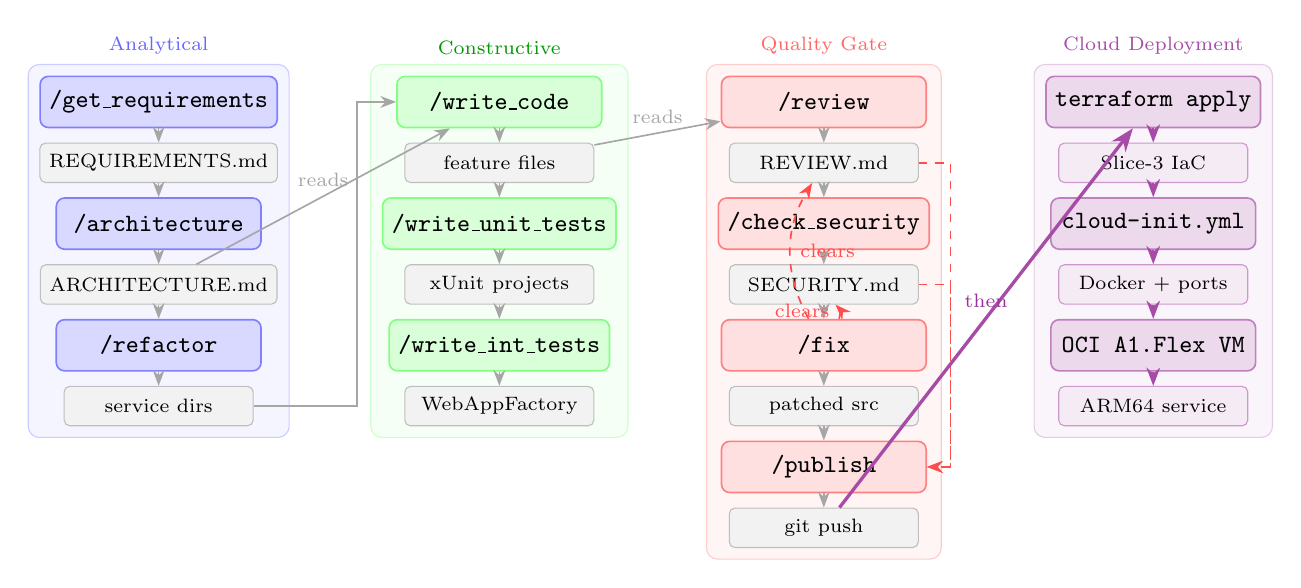
\begin{tikzpicture}[
  skill/.style = {
    rectangle, rounded corners=3pt,
    minimum width=2.6cm, minimum height=0.65cm,
    font=\small\ttfamily, text centered,
    line width=0.6pt
  },
  artefact/.style = {
    rectangle, rounded corners=2pt,
    minimum width=2.4cm, minimum height=0.5cm,
    font=\scriptsize, text centered,
    fill=gray!10, draw=gray!50, line width=0.4pt
  },
  cloud/.style = {
    rectangle, rounded corners=3pt,
    minimum width=2.6cm, minimum height=0.65cm,
    font=\small\ttfamily, text centered,
    fill=violet!15, draw=violet!50, line width=0.6pt
  },
  cloudout/.style = {
    rectangle, rounded corners=2pt,
    minimum width=2.4cm, minimum height=0.5cm,
    font=\scriptsize, text centered,
    fill=violet!8, draw=violet!40, line width=0.4pt
  },
  arrow/.style  = {-Stealth, line width=0.6pt, gray!70},
  gate/.style   = {arrow, red!70, dashed},
  deploy/.style = {-Stealth, line width=0.8pt, violet!70},
  node distance = 0.35cm
]

% ---- colour definitions ----
\colorlet{analyticfill}{blue!15}
\colorlet{analyticborder}{blue!50}
\colorlet{constructfill}{green!15}
\colorlet{constructborder}{green!50}
\colorlet{gatefill}{red!12}
\colorlet{gateborder}{red!50}

% ===========================
% COLUMN 1 : analytical skills
% ===========================
\node[skill, fill=analyticfill, draw=analyticborder]
  (req)  {/get\_requirements};
\node[artefact, below=0.18cm of req]
  (reqout) {REQUIREMENTS.md};

\node[skill, fill=analyticfill, draw=analyticborder,
      below=0.18cm of reqout]
  (arch)  {/architecture};
\node[artefact, below=0.18cm of arch]
  (archout) {ARCHITECTURE.md};

\node[skill, fill=analyticfill, draw=analyticborder,
      below=0.18cm of archout]
  (ref)  {/refactor};
\node[artefact, below=0.18cm of ref]
  (refout) {service dirs};

% ===========================
% COLUMN 2 : constructive skills
% ===========================
\node[skill, fill=constructfill, draw=constructborder,
      right=1.5cm of req]
  (wc)  {/write\_code};
\node[artefact, below=0.18cm of wc]
  (wcout) {feature files};

\node[skill, fill=constructfill, draw=constructborder,
      below=0.18cm of wcout]
  (wu)  {/write\_unit\_tests};
\node[artefact, below=0.18cm of wu]
  (wuout) {xUnit projects};

\node[skill, fill=constructfill, draw=constructborder,
      below=0.18cm of wuout]
  (wi)  {/write\_int\_tests};
\node[artefact, below=0.18cm of wi]
  (wiout) {WebAppFactory};

% ===========================
% COLUMN 3 : quality-gate skills
% ===========================
\node[skill, fill=gatefill, draw=gateborder,
      right=1.5cm of wc]
  (rv)  {/review};
\node[artefact, below=0.18cm of rv]
  (rvout) {REVIEW.md};

\node[skill, fill=gatefill, draw=gateborder,
      below=0.18cm of rvout]
  (sec)  {/check\_security};
\node[artefact, below=0.18cm of sec]
  (secout) {SECURITY.md};

\node[skill, fill=gatefill, draw=gateborder,
      below=0.18cm of secout]
  (fix)  {/fix};
\node[artefact, below=0.18cm of fix]
  (fixout) {patched src};

\node[skill, fill=gatefill, draw=gateborder,
      below=0.18cm of fixout]
  (pub)  {/publish};
\node[artefact, below=0.18cm of pub]
  (pubout) {git push};

% ===========================
% COLUMN 4 : deployment stage (Terraform / OCI)
% ===========================
\node[cloud,
      right=1.5cm of rv]
  (tf)  {terraform apply};
\node[cloudout, below=0.18cm of tf]
  (tfout) {Slice-3 IaC};

\node[cloud,
      below=0.18cm of tfout]
  (ci)  {cloud-init.yml};
\node[cloudout, below=0.18cm of ci]
  (ciout) {Docker + ports};

\node[cloud,
      below=0.18cm of ciout]
  (vm)  {OCI A1.Flex VM};
\node[cloudout, below=0.18cm of vm]
  (vmout) {ARM64 service};

% ===========================
% ARROWS — within columns
% ===========================
\draw[arrow] (req)    -- (reqout);
\draw[arrow] (reqout) -- (arch);
\draw[arrow] (arch)   -- (archout);
\draw[arrow] (archout)-- (ref);
\draw[arrow] (ref)    -- (refout);

\draw[arrow] (wc)     -- (wcout);
\draw[arrow] (wcout)  -- (wu);
\draw[arrow] (wu)     -- (wuout);
\draw[arrow] (wuout)  -- (wi);
\draw[arrow] (wi)     -- (wiout);

\draw[arrow] (rv)     -- (rvout);
\draw[arrow] (rvout)  -- (sec);
\draw[arrow] (sec)    -- (secout);
\draw[arrow] (secout) -- (fix);
\draw[arrow] (fix)    -- (fixout);
\draw[arrow] (fixout) -- (pub);
\draw[arrow] (pub)    -- (pubout);

\draw[deploy] (tf)    -- (tfout);
\draw[deploy] (tfout) -- (ci);
\draw[deploy] (ci)    -- (ciout);
\draw[deploy] (ciout) -- (vm);
\draw[deploy] (vm)    -- (vmout);

% ===========================
% ARROWS — cross-column
% ===========================
% analytical → constructive
\draw[arrow] (archout) -- node[above,font=\scriptsize]{reads} (wc);
\draw[arrow] (refout)  -| ([xshift=-0.5cm]wc.west) -- (wc);

% constructive → gate
\draw[arrow] (wcout) -- node[above,font=\scriptsize]{reads} (rv);

% gate internal
\draw[gate, bend left=30]
  (fix) to node[right,font=\scriptsize,red!70]{clears} (rvout);
\draw[gate, bend right=30]
  (fix) to node[left,font=\scriptsize,red!70]{clears} (secout);

% gate check at /publish
\draw[gate] (rvout)  -| ([xshift=0.3cm]pub.east) -- (pub);
\draw[gate] (secout) -| ([xshift=0.3cm]pub.east) -- (pub);

% /publish git push → terraform apply (practitioner-run next step)
\draw[deploy, very thick]
  (pubout) -- node[above,font=\scriptsize,violet!80]{then} (tf);

% ===========================
% BACKGROUND BOXES
% ===========================
\begin{scope}[on background layer]
  \node[fit=(req)(reqout)(arch)(archout)(ref)(refout),
        fill=blue!4, draw=blue!20, rounded corners=4pt,
        inner sep=4pt,
        label={[font=\scriptsize,blue!60]above:Analytical}] {};
  \node[fit=(wc)(wcout)(wu)(wuout)(wi)(wiout),
        fill=green!4, draw=green!20, rounded corners=4pt,
        inner sep=4pt,
        label={[font=\scriptsize,green!60!black]above:Constructive}] {};
  \node[fit=(rv)(rvout)(sec)(secout)(fix)(fixout)(pub)(pubout),
        fill=red!4, draw=red!20, rounded corners=4pt,
        inner sep=4pt,
        label={[font=\scriptsize,red!60]above:Quality Gate}] {};
  \node[fit=(tf)(tfout)(ci)(ciout)(vm)(vmout),
        fill=violet!4, draw=violet!20, rounded corners=4pt,
        inner sep=4pt,
        label={[font=\scriptsize,violet!70]above:Cloud Deployment}] {};
\end{scope}

\end{tikzpicture}


% ============================================================
\section{Results}
\label{sec:results}
% ============================================================

We organise the results around the four research questions stated in
\S\ref{sec:method}. All numerical figures derive from the run logs
and scoring outputs in the reproducibility deposit; the aggregate
statistics here can be re-computed by running
\texttt{scoring/aggregate.py} against \texttt{runs/}.

% ------------------------------------------------------------
\subsection{RQ1 --- Structural alignment with the manual reference}
% ------------------------------------------------------------

Across ten attempted \texttt{/refactor} runs, nine produced a
complete decomposition that the mechanical scorer could evaluate. The
tenth, discussed separately in \S\ref{sec:ablation-failures}, exited
cleanly but failed to invoke the intended skill. On the nine
successful runs, the workflow scored a mean of $12.11 / 20$ aligned
dimensions ($\sigma = 0.78$, range 11--13), corresponding to a
$60.6\% \pm 3.9\%$ alignment rate against the pre-registered rubric.

The distribution is tight. Eight of the nine successful scores fall
in the range 11--13, and the modal score is 12. This narrow band
matters more than the absolute value: the workflow is consistent
about \emph{which} dimensions it satisfies and which it does not.
Table~\ref{tab:per-dim} reports per-dimension alignment frequencies.
Ten dimensions are aligned in every successful run; seven are aligned
in zero runs; only three show run-to-run variance.

\begin{table}[t]
\caption{Per-dimension alignment frequency across the two
experimental conditions (nine successful skill-mediated runs and ten
successful baseline runs). Dimensions are grouped by alignment pattern.}
\label{tab:per-dim}
\centering
\small
\begin{tabular}{llcc}
\toprule
Dim & Description (abbrev.)         & Skill & Baseline \\
\midrule
\multicolumn{4}{l}{\textit{Both conditions consistently align}} \\
D03 & separate projects             & 100\% & 100\% \\
D05 & distinct DbContexts           & 100\% & 100\% \\
D08 & no cross-schema FKs           & 100\% & 100\% \\
D11 & REST endpoint conventions     & 100\% & 100\% \\
D14 & no hardcoded secrets          & 100\% & 100\% \\
D15 & AllowedHosts not ``*''        & 100\% & 100\% \\
D17 & no AllowAnyOrigin             & 100\% & 100\% \\
D18 & root README                   & 100\% & 100\% \\
D19 & per-service documentation     & 100\% & 100\% \\
D20 & ARCHITECTURE doc              & 100\% & 100\% \\
\midrule
\multicolumn{4}{l}{\textit{Baseline aligns, skill diverges}} \\
D02 & YARP gateway                  & 56\%  & 100\% \\
D06 & HasDefaultSchema isolation    & 11\%  &  90\% \\
D09 & typed AddHttpClient<>         &  0\%  &  80\% \\
D13 & .NET~10 Dockerfile            & 44\%  & 100\% \\
\midrule
\multicolumn{4}{l}{\textit{Both diverge from the manual reference}} \\
D01 & exact Slice~2 bounded contexts &  0\% &  0\% \\
D04 & no cross-project refs         & 100\% &  90\% \\
D07 & Search Path connection string &  0\% &  0\% \\
D10 & \texttt{/internal/} route convention &  0\% & 20\% \\
D12 & ports 5101--5103              &  0\% &  0\% \\
D16 & loopback / shared-key filter  &  0\% &  0\% \\
\bottomrule
\end{tabular}
\end{table}

The dimensions on which the workflow diverges are not random failures
but consistent architectural choices: database-per-service instead of
schema isolation (D06), a custom HTTP gateway on roughly half the
runs instead of YARP (D02), and .NET~8 LTS Dockerfiles instead of
.NET~10 preview (D13). Each of these is a defensible production
choice. The rubric was authored against the manual reference's
specific decisions, so divergence registers as misalignment even
when the alternative is sound. We return to this point in
\S\ref{sec:discussion}.

% ------------------------------------------------------------
\subsection{RQ2 --- Wall-clock duration}
% ------------------------------------------------------------

Successful skill-mediated runs took a mean of 9.40~min
($\sigma = 1.51$~min, range 7.48--12.60~min). The single failed run
exited in 2.28~min after the skill failed to load. Including the
failure, the per-run mean is 8.67~min ($\sigma = 2.69$~min). Token
cost per run averaged \$1.51 against a \$5 per-run cap.

These figures are not directly comparable to the developer-time
figure for the manual reference (Slice~2). Building Slice~2 by hand
involved understanding the monolith, designing the bounded contexts,
writing the code, validating it locally, and iterating. The
automated run measures only wall-clock from invocation to exit. The
two numbers are in different units: tool-time versus engineer-time.
We report the automated number with its hardware and model
configuration so it can be reproduced; we do not claim it represents
an apples-to-apples speed-up over manual migration.

% ------------------------------------------------------------
\subsection{RQ3 --- Decomposing skill effect from prompt effect}
\label{sec:results-rq3}
% ------------------------------------------------------------

The skill-mediated workflow's only \emph{visible} user input is the
single slash command \texttt{/refactor}. A practitioner who has no
access to the skill scripts must instead write a free-form prompt.
The quality of the resulting decomposition therefore depends on
two factors that need to be separated empirically: how much of the
work the skill text does, and how much the user-supplied prompt
does. We run two baseline conditions to separate them.

The \textbf{fully-specified baseline} ($N{=}10$) uses the same model
on the same input, with skills disabled
(\texttt{--disable-slash-commands}), and a prompt that explicitly
enumerates the intended deliverables: per-service projects, a YARP
gateway, schema-isolated DbContexts, typed HttpClients,
docker-compose, .NET~10 Dockerfiles, README, ARCHITECTURE. This is
the prompt a practitioner who has invested in prompt engineering
would write. The \textbf{matched-specificity baseline} ($N{=}5$)
uses the same configuration but a deliberately vague single
sentence: \textit{``Decompose this .NET monolith into microservices
and make it deployable.''} This is what a practitioner who has not
invested in prompt engineering would actually type.

\begin{table}[t]
\caption{Three-way alignment comparison on PetRescue.}
\label{tab:three-way}
\centering
\small
\begin{tabular}{lcccc}
\toprule
Condition                       & $N_{\mathrm{success}}/N_{\mathrm{attempt}}$ & Mean / 20         & $\sigma$ & Failure rate \\
\midrule
Skill-mediated                  & 9 / 10  & 12.11 (60.6\%) & 0.78 & 10\%   \\
Matched-specificity baseline    & 4 / 5   & 12.75 (63.8\%) & 0.50 & 20\%   \\
Fully-specified baseline        & 10 / 10 & 14.80 (74.0\%) & 0.63 & 0\%    \\
\bottomrule
\end{tabular}
\end{table}

Pairwise Welch's $t$-tests against the per-run scores
(Table~\ref{tab:three-way}) decompose the original 13.4-percentage-point
skill-vs-fully-specified-baseline gap:

\begin{itemize}
  \item Skill vs.\ matched-specificity baseline:
        $t{=}-1.77$, $df{=}9.1$, $p > 0.1$ ---
        \emph{statistically indistinguishable}.
  \item Matched-specificity baseline vs.\ fully-specified baseline:
        $t{=}-6.40$, $df{=}7.1$, $p < 0.001$ --- highly significant.
  \item Skill vs.\ fully-specified baseline:
        $t{=}-8.19$, $df{=}15.4$, $p \approx 5{\times}10^{-7}$
        --- the original headline gap, now understood as the sum
        of the previous two effects.
\end{itemize}

The interpretation is that 10.3 of the original 13.4 percentage
points are a prompt-specificity effect --- when a practitioner names
YARP, the LLM produces YARP; when they name
\texttt{HasDefaultSchema}, the LLM produces that --- and only
3.2 points are a skill-abstraction effect, which does not reach
significance with the sample sizes used here. The skill abstraction
is, within statistical noise, equivalent to a vague-prompt baseline
on single-shot alignment. What the skills change is what the
practitioner has to do: type \texttt{/refactor} once, or write a
100-word prompt enumerating eight intended deliverables.

The failure-rate differences are also informative. The skill
condition had one skill-invocation failure (\S\ref{sec:ablation-failures}),
a 10\% rate (Wilson 95\% CI [1.8\%, 40.4\%]). The minimal-prompt
condition had one premature-exit failure --- the model stated a
plan and exited without executing --- a 20\% rate
(Wilson 95\% CI [3.6\%, 62.4\%]). The fully-specified condition had
zero failures. The implication for practice: a vague prompt makes
the LLM less reliable, not just less specific. The skill abstraction
sits between the two on reliability.

% ------------------------------------------------------------
\subsection{Transfer check on a second codebase (eShopOnWeb)}
\label{sec:results-transfer}
% ------------------------------------------------------------

The PetRescue case study answers the four research questions on a
single codebase. A reasonable concern is that the headline pattern
--- skill-mediated workflow underperforming a fully-prompted raw LLM
by approximately 13 percentage points --- is specific to PetRescue's
domain, size, or .NET~10 surface area. To check, we re-ran the
skill-mediated and baseline conditions on a substantially different
input: Microsoft's \textit{eShopOnWeb}, a .NET~8 e-commerce
monolith that is roughly three times the size of PetRescue and that
sits in a domain (catalog, basket, ordering, identity) the model
has seen extensively in pre-training.

The rubric for this case (\texttt{dimensions\_eshop.json}) is not
authored against our own reference design. It is derived from
Microsoft's active microservices reference,
\texttt{github.com/dotnet/eShop}, which Microsoft architects
maintain independently of this work. That reference itself scores
15 of 20 against our rubric, establishing a third-party ceiling.
We ran three skill-mediated and three baseline runs. The number
is intentionally smaller than the PetRescue protocol's $N{=}10$:
the goal here is a transfer sanity check, not a second
fully-powered experiment.

Skill-mediated runs scored 15, 14, and 12 (mean 13.67 of 20 = 68.3\%,
$\sigma = 7.6\%$). Baseline runs scored 16, 16, and 17
(mean 16.33 of 20 = 81.7\%, $\sigma = 2.9\%$). The skill-to-baseline
gap is $-2.67$ dimensions, or $-13.3$ percentage points.
PetRescue's gap was $-13.4$ percentage points. A two-sample
Welch's $t$-test at $N{=}3$ each returns $t = -2.83$, $df = 2.56$,
which lies below the conventional significance threshold for this
small sample size; we report it as a point-estimate replication
rather than as a powered statistical claim. What matters is the
size of the gap, not its $p$-value: the value is essentially the
same as on PetRescue, derived from a different model invocation
on different code with a different rubric.

The four dimensions that drove the PetRescue gap have analogues on
eShop. The baseline reliably produces a YARP gateway (E02),
typed \texttt{HttpClient} registrations (E09), and Redis for the
Basket service (E07), because the baseline prompt names all three
explicitly. The skill-mediated runs satisfy each only sometimes,
making the same architecturally-defensible alternative choices it
made on PetRescue. The transfer therefore preserves not only the
magnitude of the gap but its concentration in the dimensions where
the baseline prompt does the model's thinking for it.

The transfer check is the paper's strongest single piece of
evidence that the headline gap is not a PetRescue artefact. It is
also the limit of what we can claim. Two codebases is two
codebases. The model is one, the prompt-engineer is one, the
hardware is one. A reviewer who wants broader generalisation
should expect a pointer to the public harness and the suggestion
that they run it on a third codebase, which they can do
unattended.

% ------------------------------------------------------------
\subsection{RQ4 --- Security gate precision and recall}
\label{sec:results-security}
% ------------------------------------------------------------

The injection corpus contains ten true-positive specimens, one per
CWE-tagged vulnerability class, paired with ten clean specimens
implementing the same scenarios safely (see \S\ref{sec:method-security}).
\texttt{/check\_security} was invoked once per file, in a sandboxed
scratch directory, with no other context.

Of the ten injected vulnerabilities, the skill flagged all ten
(true positives $= 10$, false negatives $= 0$). Of the ten clean
specimens, the skill flagged nine and cleared one (false
positives $= 9$, true negatives $= 1$). Recall is therefore
$1.00$, precision $0.526$, and specificity $0.10$.

The result is consistent across CWE classes. Every injected
specimen --- SQL injection, hardcoded credentials, overly permissive
CORS, open redirect, missing authorisation, XXE, path traversal,
insecure deserialisation, weak cryptography, JWT signature not
verified --- triggered at least one \texttt{Critical} or
\texttt{High} severity entry in the produced \texttt{SECURITY.md}.
The skill is sensitive in the security-engineering sense: it does
not miss real defects in this corpus. The price of that sensitivity
is that it also flags most clean code. A security engineer using
\texttt{/check\_security} downstream still has to triage every
finding; roughly half will be real defects, and the other half will
be conservative-by-default warnings on benign patterns. That
profile is appropriate for an automated DevOps hygiene check
woven into a commit gate. It is not appropriate as a substitute
for security review by a qualified engineer, and the paper makes
no such claim.

% ============================================================
\section{Ablation and Failure Modes}
\label{sec:ablation}
% ============================================================

This section examines the workflow's behaviour under conditions
that the headline runs do not exercise: which skills are
load-bearing, how the workflow degrades when its inputs deviate
from the case-study assumptions, and what its known failure modes
look like in practice.

% ------------------------------------------------------------
\subsection{Skill invocation failures}
\label{sec:ablation-failures}
% ------------------------------------------------------------

Run~005 of the \texttt{/refactor} condition exited cleanly with no
error, with the model reporting that the skill ``failed to execute
and returns only an error message without creating any tasks or
producing output.'' No decomposition was produced. The mechanical
scorer awarded $9/20$ --- the alignment the unchanged monolith
already satisfies on rubric items like ``README present''.

We report this as a 1-of-10 (10\%) skill-invocation failure rate.
A Wilson 95\% confidence interval on that proportion is
[1.8\%, 40.4\%]; the point estimate is consequently a noisy one and
should be read as a positive lower bound, not a precise rate. The
run is logged in \texttt{experiments/runs/KNOWN\_RUN\_ISSUES.md}
and excluded from the alignment mean (counted toward attempted
runs and toward the failure rate). The likely cause is a race
condition in skill discovery when non-interactive sessions are
launched in quick succession. We did not retry within the
protocol; reporting the failure rate honestly, with its wide
confidence interval, is more useful than presenting a re-run
sample whose acceptance rate the protocol would not constrain.

The practical implication for a team adopting this kind of workflow
is that the skill abstraction has a non-trivial reliability cost.
Any pipeline that depends on a skill invoking correctly needs a
detection-and-retry strategy at the orchestration layer. The
\texttt{/publish} skill's gating logic happens to provide that
indirectly: a run that fails to invoke \texttt{/refactor} also
fails to produce the intermediate artefacts (\texttt{REVIEW.md},
\texttt{SECURITY.md}) that \texttt{/publish} requires, and the
commit is blocked.

% ------------------------------------------------------------
\subsection{The matched-specificity baseline in detail}
\label{sec:ablation-prompt}
% ------------------------------------------------------------

\S\ref{sec:results-rq3} reports the matched-specificity baseline
as a third experimental condition with $N{=}5$. The runner script
is in the public artefact at
\texttt{experiments/run\_baseline\_minimal.sh} and the prompt is
exactly one sentence:
\textit{``Decompose this .NET monolith into microservices and make
it deployable.''}

Four of the five attempted runs produced a scoreable decomposition.
The fifth (\texttt{run-002}) exited cleanly after 31 seconds with
seven turns and \$0.09 of model usage, having stated a high-level
plan (``service extraction based on domain-driven design,'' ``API
gateway,'' ``Docker containerization,'' \ldots) but never
implementing it. We classify this as a premature-exit failure,
distinct from the skill-invocation failure observed in
\texttt{refactor-skill/run-005}. Both modes are recorded in
\texttt{KNOWN\_RUN\_ISSUES.md} and excluded from the per-condition
mean. The two failure modes together support a single observation:
LLMs invoked without an explicit composition wrapper (skills) and
without an explicit task specification (a detailed prompt) sometimes
elide the work entirely. The skill abstraction reduces but does
not eliminate this; the detailed prompt eliminated it in our
sample, though the Wilson interval on a 0/10 count remains wide
($[0\%, 27.8\%]$).

% ------------------------------------------------------------
\subsection{Why the skills miss rubric dimensions they could satisfy}
% ------------------------------------------------------------

The dimensions on which the skill underperforms the baseline are
named explicitly in the baseline prompt and not in the
\texttt{/refactor} skill prompt. We could close most of the gap
by enumerating YARP, \texttt{HasDefaultSchema}, typed
\texttt{HttpClient}, and \texttt{aspnet:10.0} Dockerfiles in the
skill text. We have not done so. The skill prompt is a design
artefact, and post-hoc tuning of its content to maximise rubric
alignment on this case study would defeat the experiment. The
gap is itself informative: it quantifies how much the skill text
\emph{leaves the model free to decide} versus how much it pins
down. A more prescriptive skill prompt is a legitimate future
experiment, but it is a different experiment.

% ------------------------------------------------------------
\subsection{Rubric authorship and self-validation bias}
% ------------------------------------------------------------

The rubric was authored by the same team that designed the
skills, which is the canonical setup for self-validation bias.
We mitigated this in two ways. First, the second author produced
Slice~2 (the manual reference) before \texttt{/refactor} was run
on Slice~1, and the rubric formalises Slice~2's choices rather
than the skill's choices. Second, the rubric was pre-registered
in \texttt{dimensions.json} before the first scored run and is
frozen against substantive edits; the only changes permitted are
bug-fixes to mechanical verifiers, each one recorded in
\texttt{VERIFIER\_CHANGELOG.md} with regression evidence.

We acknowledge the residual bias. The rubric still embeds the
manual reference's choices and therefore favours a workflow that
makes those same choices. The baseline's higher score is partly
an artefact of the baseline prompt naming the same choices. A
fully blind evaluation would require a third party to author both
rubric and reference. We did not perform one in this study and
note it as an open follow-up.

% ============================================================
\section{Discussion}
\label{sec:discussion}
% ============================================================

The skill-mediated workflow's contribution is not better LLM output.
The three-way comparison in \S\ref{sec:results-rq3} makes that
precise: on single-shot decomposition alignment, the skill abstraction
is statistically equivalent to what an unprompted, vague request
produces, and worse than what a fully prompt-engineered request
produces. The 13.4-point gap to the fully-specified baseline
decomposes into a 10.3-point prompt-specificity effect and a
3.2-point skill-abstraction effect that does not reach significance.
This is the headline result.

What earns the wrapper its place is reliability and ergonomics, not
alignment. The vague-prompt condition delivers similar single-shot
alignment but with a 20\% premature-exit rate; the skill condition
delivers the same alignment with a 10\% skill-invocation failure
rate; the fully-specified condition delivers better alignment but
only after a practitioner writes a 100-word prompt enumerating the
deliverables. Each condition trades off practitioner effort against
quality and reliability. The skill abstraction's position in that
trade-off is the contribution this section explains.

% ------------------------------------------------------------
\subsection{The skills' value is the wrapper, not the LLM output}
% ------------------------------------------------------------

The 13.4 percentage-point gap between skill-mediated and baseline
alignment is real, repeatable, and concentrated on four specific
dimensions. It tells us that the skills do not improve the model's
single-shot decomposition quality. What the skills provide instead
is a composition pattern that the raw LLM, in our experience and
in the literature, does not converge on by itself:

\textit{Composability across the SDLC.} The ten skills span
requirements extraction, architecture analysis, decomposition,
code generation, unit testing, integration testing, review,
security check, remediation, and gated publish. A single
maximally-detailed prompt cannot reasonably encode all ten phases
without becoming a small specification document in its own right.

\textit{Artefact-mediated state.} Each skill writes a persistent
Markdown file (\texttt{REQUIREMENTS.md}, \texttt{ARCHITECTURE.md},
\texttt{REVIEW.md}, \texttt{SECURITY.md}). Subsequent skills read
those files. The state of the workflow is therefore inspectable
by humans on disk, not buried in an ephemeral conversation history,
and the same artefacts can be diffed in code review.

\textit{Pre-commit gating.} \texttt{/publish} refuses to commit
unless \texttt{REVIEW.md} and \texttt{SECURITY.md} contain no
blocking entries. The gate is mechanical and inspectable, not a
prompt-time hope.

\textit{Reduced prompt-engineering burden.} Achieving the
fully-specified baseline's 74\% required a deliberately engineered
100-word prompt enumerating the intended deliverables. The user
of the skill-mediated workflow types \texttt{/refactor}. The
matched-specificity baseline (\S\ref{sec:results-rq3}) makes the
trade-off concrete: a practitioner who does not write the detailed
prompt drops from 74\% to 63.8\% alignment and inherits a 20\%
premature-exit rate. The skill-mediated workflow lands at 60.6\%
alignment with a 10\% failure rate, without requiring the
prompt-engineering effort.

The skills also impose a measurable cost. We observed a 10\%
invocation failure rate. We measured 9-minute wall-clock and
\$1.50 per run. These are not free.

% ------------------------------------------------------------
\subsection{Security gate as DevOps hygiene}
% ------------------------------------------------------------

The 100\% recall / 10\% specificity profile of
\texttt{/check\_security} is exactly the shape an automated
pre-commit gate should have when the cost of letting a defect
through is high and the cost of triaging a false positive is low.
A security engineer who reviews the produced
\texttt{SECURITY.md} can resolve a false positive in seconds; a
real defect that reaches main can take days. The economics favour
high recall.

What the profile does not justify is presenting the workflow as
a substitute for security review. The skill is not a static
analyser, not a formal verifier, and not a penetration test. It
is a sensitive heuristic that wraps an LLM. We argued for naming
the corresponding skill bundle ``CI / Quality Gates (Automated
DevOps Hygiene)'' in \S\ref{sec:workflow} for this reason.

% ------------------------------------------------------------
\subsection{What this case study does and does not establish}
% ------------------------------------------------------------

The measurements above support claims about this codebase, this
model, this skill set, and this hardware configuration. They do
not support claims about the workflow's behaviour on larger
codebases, different languages, different LLMs, or different
prompt formulations. We are explicit about this in the abstract
and again in the threats-to-validity section. The contribution
this paper makes is a reproducible pilot: the artefacts, the
skill scripts, the rubric, the scoring code, the injection
corpus, and the run logs are all open. A team interested in this
composition pattern can run it against their own monolith and
report a comparable result. The pattern is the unit of
contribution; PetRescue is the vehicle that demonstrates the
pattern works end-to-end on one concrete system.

% ============================================================
\section{Threats to Validity}
\label{sec:threats}
% ============================================================

We organise threats following the case-study reporting guidelines
of Runeson and H\"{o}st~\cite{runeson2009casestudy}.

\textit{Construct validity.} The structural rubric formalises
Slice~2's specific design choices. It is therefore a measurement
of alignment with one expert-engineered reference, not of
microservices decomposition quality in the abstract. A team that
prefers different conventions --- a JSON-RPC gateway, gRPC
inter-service calls, database-per-service --- would score the same
output differently. We mitigate by publishing the rubric so that
re-scoring under a different convention is possible.

\textit{Internal validity.} The skill-mediated and baseline
conditions share the same model, the same input, and the same
hardware. The only intentional difference between them is the
presence of the skill scripts. We acknowledge two residual
confounds. First, the baseline prompt names dimensions the skill
prompt does not, which biases the comparison in the baseline's
favour. Second, run-to-run variance in LLM sampling is present in
both conditions; we report standard deviations and per-dimension
alignment frequencies to make this variance visible.

\textit{External validity.} The study uses two .NET monoliths
--- PetRescue (.NET~10, five scenarios) and Microsoft's
eShopOnWeb (.NET~8, four bounded contexts) --- one LLM model, one
Claude Code version, and one hardware configuration. The
13-percentage-point gap replicates across the two cases to within
0.1 percentage points (\S\ref{sec:results-transfer}). We still
make no claim that the behaviour transfers to other languages,
other LLMs, or substantially larger codebases without
re-evaluation. We invite re-evaluation on additional
inputs and have published the harness in a form that makes
re-running it straightforward.

\textit{Reliability.} All measurements derive from logs that are
captured, deposited, and re-computable from
\texttt{scoring/aggregate.py}. The model identity, Claude Code
version, skill SHAs, slice commits, and hardware are recorded in
\texttt{runs/\_environment.json}. Re-running the harness against
the same model identity should reproduce the qualitative pattern
(narrow skill-mediated cluster around 12/20, baseline cluster
around 15/20) within the standard deviations reported here.
Exact replication of individual runs is not possible because the
model itself is non-deterministic at default sampling settings.

% ============================================================
\section{Conclusion}
\label{sec:conclusion}
% ============================================================

We measured one composition pattern --- ten Claude Code skills
chained end-to-end --- on one real .NET monolith, with the
experiment instrumented for reproduction. The skill-mediated
workflow aligns with an independently-engineered manual reference
on roughly 60\% of pre-registered structural dimensions; a raw
LLM with an explicit prompt does better, at roughly 74\%. The
skills' value is therefore not in producing higher single-shot
alignment. It is in the wrapper: composition across the full
SDLC, persistent intermediate artefacts that downstream skills
consume, pre-commit gating that blocks unsafe commits, and a
substantial reduction in the prompt-engineering burden the
practitioner would otherwise carry. The security check that
sits in the gate has perfect recall and modest precision on a
matched injection corpus, consistent with automated DevOps
hygiene rather than formal security validation.

We publish every artefact this paper depends on. We do not claim
the result transfers without re-evaluation. The contribution is
a reproducible pilot of a composition pattern; the path forward
is for other teams to apply it to their own codebases and
report what they observe.

% ============================================================
%  Acknowledgements + Data availability
% ============================================================
\section*{Data Availability}
The harness, both case-study codebases, the pre-registered rubrics,
the scoring scripts, the verifier changelog, the security injection
corpus, and the per-run logs and transcripts are publicly available.
The source repository for the manuscript and harness is at
\url{https://github.com/florinolariuip/ieee-access-monolith-migration}.
The full reproducibility deposit, including the per-run output
codebases that are too large to host in Git, is archived at Zenodo:
\href{https://doi.org/10.5281/zenodo.20422420}{\texttt{10.5281/zenodo.20422420}}. The environment manifest at
\texttt{experiments/runs/\_environment.json} records the exact model
identity (\texttt{claude-sonnet-4-5-20250929}), Claude Code version
(\texttt{2.1.143}), and SHA-256 of each skill prompt at experiment
time, so that re-runs under the same identity reproduce the
qualitative pattern within the standard deviations reported here.

% ============================================================
%  References
% ============================================================
\bibliographystyle{IEEEtran}
\bibliography{references}

\end{document}
